\section[Analisi Rischi]{Analisi Rischi}

\subsection[Variazione Tasso Cambio]{Variazione Tasso Cambio}

\begin{longtable}{p{3cm}D{,}{,}{5.2}}
% didascalia ed etichetta
\caption{Andamento Tasso di Cambio (\euro -LEK)}\\
% intestazione iniziale
\toprule
	\makebox[3cm][c]{\textbf{Data}} & \multicolumn{1}{c}{\textbf{LEK}} \\
\midrule
\endfirsthead
% intestazione normale
\multicolumn{2}{l}{\footnotesize\itshape\tablename~\thetable:
continua dalla pagina precedente} \\
\toprule
	\makebox[3cm][c]{\textbf{Data}} & \multicolumn{1}{c}{\textbf{LEK}} \\
\midrule
\endhead
% piede normale
\midrule
\multicolumn{2}{r}{\footnotesize\itshape\tablename~\thetable:
continua nella prossima pagina} \\
\endfoot
% piede finale
\bottomrule
\multicolumn{2}{r}{\footnotesize\itshape\tablename~\thetable:
si conclude dalla pagina precedente} \\
\endlastfoot
% corpo della tabella
	\makebox[3cm][c]{$07/07/2016$} & 136,78\\
	\makebox[3cm][c]{$08/07/2016$} & 136,54\\	
 	\makebox[3cm][c]{$10/07/2016$} & 136,55\\
	\makebox[3cm][c]{$11/07/2016$} & 136,68\\
	\makebox[3cm][c]{$12/07/2016$} & 136,73\\	
 	\makebox[3cm][c]{$13/07/2016$} & 136,83\\
 	\makebox[3cm][c]{$14/07/2016$} & 136,77\\
	\makebox[3cm][c]{$15/07/2016$} & 136,52\\	
 	\makebox[3cm][c]{$17/07/2016$} & 136,53\\
	\makebox[3cm][c]{$18/07/2016$} & 136,57\\	
 	\makebox[3cm][c]{$19/07/2016$} & 136,43\\
 	\makebox[3cm][c]{$20/07/2016$} & 136,40\\
	\makebox[3cm][c]{$21/07/2016$} & 135,95\\	
 	\makebox[3cm][c]{$22/07/2016$} & 135,18\\
 	\makebox[3cm][c]{$24/07/2016$} & 135,17\\
	\makebox[3cm][c]{$25/07/2016$} & 135,98\\	
 	\makebox[3cm][c]{$26/07/2016$} & 136,34\\
 	\makebox[3cm][c]{$27/07/2016$} & 137,15\\
	\makebox[3cm][c]{$28/07/2016$} & 136,18\\	
 	\makebox[3cm][c]{$29/07/2016$} & 138,62\\
  	\makebox[3cm][c]{$31/07/2016$} & 136,12\\
	\makebox[3cm][c]{$01/08/2016$} & 136,11\\	
 	\makebox[3cm][c]{$02/08/2016$} & 136,80\\	
	\makebox[3cm][c]{$03/08/2016$} & 138,34\\	
	\makebox[3cm][c]{$04/08/2016$} & 136,06\\	
	\makebox[3cm][c]{$05/08/2016$} & 135,52\\	
	\makebox[3cm][c]{$07/08/2016$} & 135,55\\	
	\makebox[3cm][c]{$08/08/2016$} & 135,48\\	
	\makebox[3cm][c]{$09/08/2016$} & 136,21\\	
	\makebox[3cm][c]{$10/08/2016$} & 135,95\\	
	\makebox[3cm][c]{$11/08/2016$} & 136,01\\	
	\makebox[3cm][c]{$12/08/2016$} & 136,17\\	
	\makebox[3cm][c]{$14/08/2016$} & 136,13\\	
	\makebox[3cm][c]{$15/08/2016$} & 136,33\\	
	\makebox[3cm][c]{$16/08/2016$} & 135,77\\	
	\makebox[3cm][c]{$17/08/2016$} & 136,30\\	
	\makebox[3cm][c]{$18/08/2016$} & 137,37\\	
	\makebox[3cm][c]{$19/08/2016$} & 137,26\\	
	\makebox[3cm][c]{$21/08/2016$} & 136,62\\	
	\makebox[3cm][c]{$22/08/2016$} & 136,63\\	
	\makebox[3cm][c]{$23/08/2016$} & 136,86\\	
	\makebox[3cm][c]{$24/08/2016$} & 136,43\\	
	\makebox[3cm][c]{$25/08/2016$} & 137,22\\	
	\makebox[3cm][c]{$26/08/2016$} & 135,97\\	
	\makebox[3cm][c]{$28/08/2016$} & 135,77\\	
	\makebox[3cm][c]{$29/08/2016$} & 137,18\\	
	\makebox[3cm][c]{$30/08/2016$} & 136,64\\	
	\makebox[3cm][c]{$31/08/2016$} & 137,69\\
	\makebox[3cm][c]{$01/09/2016$} & 137,54\\
	\makebox[3cm][c]{$02/09/2016$} & 137,06\\
	\makebox[3cm][c]{$04/09/2016$} & 137,05\\
	\makebox[3cm][c]{$05/09/2016$} & 137,35\\
	\makebox[3cm][c]{$06/09/2016$} & 138,64\\
	\makebox[3cm][c]{$07/09/2016$} & 137,62\\
	\makebox[3cm][c]{$08/09/2016$} & 137,28\\
	\makebox[3cm][c]{$09/09/2016$} & 137,16\\
	\makebox[3cm][c]{$11/09/2016$} & 137,17\\
	\makebox[3cm][c]{$12/09/2016$} & 137,37\\
	\makebox[3cm][c]{$13/09/2016$} & 137,63\\
	\makebox[3cm][c]{$14/09/2016$} & 138,04\\
	\makebox[3cm][c]{$15/09/2016$} & 137,34\\
	\makebox[3cm][c]{$16/09/2016$} & 136,21\\
	\makebox[3cm][c]{$18/09/2016$} & 136,21\\
	\makebox[3cm][c]{$19/09/2016$} & 137,14\\
	\makebox[3cm][c]{$20/09/2016$} & 137,17\\
	\makebox[3cm][c]{$21/09/2016$} & 137,67\\
	\makebox[3cm][c]{$22/09/2016$} & 137,84\\
	\makebox[3cm][c]{$23/09/2016$} & 137,04\\
	\makebox[3cm][c]{$25/09/2016$} & 137,05\\
	\makebox[3cm][c]{$26/09/2016$} & 137,42\\
	\makebox[3cm][c]{$27/09/2016$} & 137,19\\
	\makebox[3cm][c]{$28/09/2016$} & 137,01\\
	\makebox[3cm][c]{$29/09/2016$} & 137,47\\
	\makebox[3cm][c]{$30/09/2016$} & 137,48\\
	\makebox[3cm][c]{$02/10/2016$} & 137,26\\
	\makebox[3cm][c]{$03/10/2016$} & 136,93\\
	\makebox[3cm][c]{$04/10/2016$} & 137,40\\
	\makebox[3cm][c]{$05/10/2016$} & 137,24\\
	\makebox[3cm][c]{$06/10/2016$} & 136,90\\
	\makebox[3cm][c]{$07/10/2016$} & 138,20\\
	\makebox[3cm][c]{$09/10/2016$} & 137,95\\
	\makebox[3cm][c]{$10/10/2016$} & 137,07\\
	\makebox[3cm][c]{$11/10/2016$} & 136,03\\
	\makebox[3cm][c]{$12/10/2016$} & 136,92\\
	\makebox[3cm][c]{$13/10/2016$} & 137,00\\
	\makebox[3cm][c]{$14/10/2016$} & 136,05\\
	\makebox[3cm][c]{$16/10/2016$} & 136,03\\
	\makebox[3cm][c]{$17/10/2016$} & 137,32\\
	\makebox[3cm][c]{$18/10/2016$} & 137,09\\
	\makebox[3cm][c]{$19/10/2016$} & 137,04\\
	\makebox[3cm][c]{$20/10/2016$} & 135,88\\
	\makebox[3cm][c]{$21/10/2016$} & 135,53\\
	\makebox[3cm][c]{$23/10/2016$} & 136,07\\
	\makebox[3cm][c]{$24/10/2016$} & 136,03\\
	\makebox[3cm][c]{$25/10/2016$} & 136,23\\
	\makebox[3cm][c]{$26/10/2016$} & 136,57\\
	\makebox[3cm][c]{$27/10/2016$} & 136,42\\
	\makebox[3cm][c]{$28/10/2016$} & 137,42\\
	\makebox[3cm][c]{$30/10/2016$} & 136,54\\
	\makebox[3cm][c]{$31/10/2016$} & 137,04\\	
	\makebox[3cm][c]{$01/11/2016$} & 137,48\\
	\makebox[3cm][c]{$02/11/2016$} & 137,06\\
	\makebox[3cm][c]{$03/11/2016$} & 136,47\\
	\makebox[3cm][c]{$04/11/2016$} & 137,19\\
	\makebox[3cm][c]{$06/11/2016$} & 136,41\\
	\makebox[3cm][c]{$07/11/2016$} & 136,66\\
	\makebox[3cm][c]{$08/11/2016$} & 136,57\\
	\makebox[3cm][c]{$09/11/2016$} & 134,87\\
	\makebox[3cm][c]{$10/11/2016$} & 136,32\\
	\makebox[3cm][c]{$11/11/2016$} & 135,98\\
	\makebox[3cm][c]{$13/11/2016$} & 136,00\\
	\makebox[3cm][c]{$14/11/2016$} & 136,00\\
	\makebox[3cm][c]{$15/11/2016$} & 135,89\\
	\makebox[3cm][c]{$16/11/2016$} & 136,05\\
	\makebox[3cm][c]{$17/11/2016$} & 134,59\\
	\makebox[3cm][c]{$18/11/2016$} & 135,38\\
	\makebox[3cm][c]{$20/11/2016$} & 135,38\\
	\makebox[3cm][c]{$21/11/2016$} & 135,80\\
	\makebox[3cm][c]{$22/11/2016$} & 135,80\\
	\makebox[3cm][c]{$23/11/2016$} & 135,94\\
	\makebox[3cm][c]{$24/11/2016$} & 135,81\\
	\makebox[3cm][c]{$25/11/2016$} & 136,11\\
	\makebox[3cm][c]{$27/11/2016$} & 136,19\\
	\makebox[3cm][c]{$28/11/2016$} & 135,73\\
	\makebox[3cm][c]{$29/11/2016$} & 136,37\\
	\makebox[3cm][c]{$30/11/2016$} & 135,68\\
	\makebox[3cm][c]{$01/12/2016$} & 135,77\\
	\makebox[3cm][c]{$02/12/2016$} & 136,05\\
	\makebox[3cm][c]{$04/12/2016$} & 134,45\\
	\makebox[3cm][c]{$05/12/2016$} & 136,84\\
	\makebox[3cm][c]{$06/12/2016$} & 137,10\\
	\makebox[3cm][c]{$07/12/2016$} & 135,81\\
	\makebox[3cm][c]{$08/12/2016$} & 135,78\\
	\makebox[3cm][c]{$09/12/2016$} & 135,86\\
	\makebox[3cm][c]{$11/12/2016$} & 135,65\\
	\makebox[3cm][c]{$12/12/2016$} & 135,81\\
	\makebox[3cm][c]{$13/12/2016$} & 135,63\\
	\makebox[3cm][c]{$14/12/2016$} & 134,65\\
	\makebox[3cm][c]{$15/12/2016$} & 135,50\\
	\makebox[3cm][c]{$16/12/2016$} & 135,73\\
	\makebox[3cm][c]{$18/12/2016$} & 135,66\\
	\makebox[3cm][c]{$19/12/2016$} & 135,17\\
	\makebox[3cm][c]{$20/12/2016$} & 134,45\\
	\makebox[3cm][c]{$21/12/2016$} & 134,37\\
	\makebox[3cm][c]{$22/12/2016$} & 134,43\\
	\makebox[3cm][c]{$23/12/2016$} & 134,35\\
	\makebox[3cm][c]{$25/12/2016$} & 134,60\\	
	\makebox[3cm][c]{$26/12/2016$} & 134,38\\
	\makebox[3cm][c]{$27/12/2016$} & 134,52\\
	\makebox[3cm][c]{$28/12/2016$} & 134,94\\
	\makebox[3cm][c]{$29/12/2016$} & 134,86\\
	\makebox[3cm][c]{$30/12/2016$} & 134,90\\
	\makebox[3cm][c]{$01/01/2017$} & 134,95\\
	\makebox[3cm][c]{$02/01/2017$} & 134,39\\				
\end{longtable}

Prendendo in esame il campione caratterizzato dai valori precedentemente esposti, si possono calcolare le seguenti statistiche di interesse:

\begin{savenotes}
\begin{table}[htb]
\centering
 \caption{Statistiche}
 \begin{tabular}{p{5cm}D{,}{,}{5.5}}
 \toprule
 	\multicolumn{1}{c}{\textbf{Statistica}} & \multicolumn{1}{c}{\textbf{Valore}} \\
 \midrule 		
	\makebox[5cm][r]{Media Campionaria} & 136,47083\\
 	\makebox[5cm][r]{Varianza Campionaria Corretta} & 0,88366\\
 	\makebox[5cm][r]{Deviazione Standard Corretta} & 0,94003\\	
 \bottomrule
 \end{tabular} 
\end{table}
\end{savenotes}

Da questi valori si può determinare il seguente intervallo di confidenza con il 95 \% di attendibilità

\[	\left [ 135,53 ; 137,41 \right]		\]

possiamo calcolare, quindi, il valore del VAN nel punto di pareggio (\euro 65355,07) con i seguenti fattori di aggiustamento del tasso di cambio in corrispondenza degli estremi dell'intervallo di confidenza preso in esame:

\begin{savenotes}
\begin{table}[htb]
\centering
 \caption{Variazione VAN}
 \begin{tabular}{D{,}{,}{5.2}D{,}{,}{4.3}D{,}{,}{7.2}D{,}{,}{7.2}}
 \toprule
 	\multicolumn{1}{c}{\textbf{Estremo Intervallo Confidenza}} & 
 	\multicolumn{1}{c}{\textbf{Aggiustamento}}			&
 	\multicolumn{2}{c}{\textbf{Valore VAN}} \\
 	& & \multicolumn{1}{c}{Punto Pareggio} & \multicolumn{1}{c}{Caso di Studio 15 \% Ottimo} \\
 \midrule 		
	135,53 & 1,007 & -4429,54 & 206380,00\\
	137,41 & 0,993 & 4639,44 & 2154498,00\\	
 \bottomrule
 \end{tabular} 
\end{table}
\end{savenotes}


\subsection[Malattia Dipendenti]{Malattia Dipendenti}

 \begin{tabular}{SS[table-format=2]}
 \toprule
 	{Anno} & {Giorni Malattia} \\
 \midrule
 	1990 & 10,7 \\
 	1991 & 11,1 \\
 	1992 & 11,1 \\
 	1993 & 11,4 \\
 	1994 & 11,4 \\
 	1995 & 11,6 \\
	1996 & 11,5 \\ 
	1997 & 11,3 \\
	1998 & 11,2 \\
	1999 & 11,5 \\
	2000 & 11,6 \\
	2001 & 11,8 \\
	2002 & 12,1 \\
	2003 & 12,2 \\
	2004 & 11,8 \\
	2006 & 11,4 \\
	2007 & 11,4 \\
	2008 & 11,6 \\
	2009 & 11,7 \\
	2010 & 11,6 \\
	2011 & 11,6 \\
	2012 & 11,7 \\							  
	2013 & 11,8 \\
	2014 & 11,8 \\

 \bottomrule
 \end{tabular} 

 La regressione calcolata è di tipo logaritmica ed e' pari a:
 
 \[ f(x) = 0,293204 * ln(12,53 * 10^{15} * x )\]

 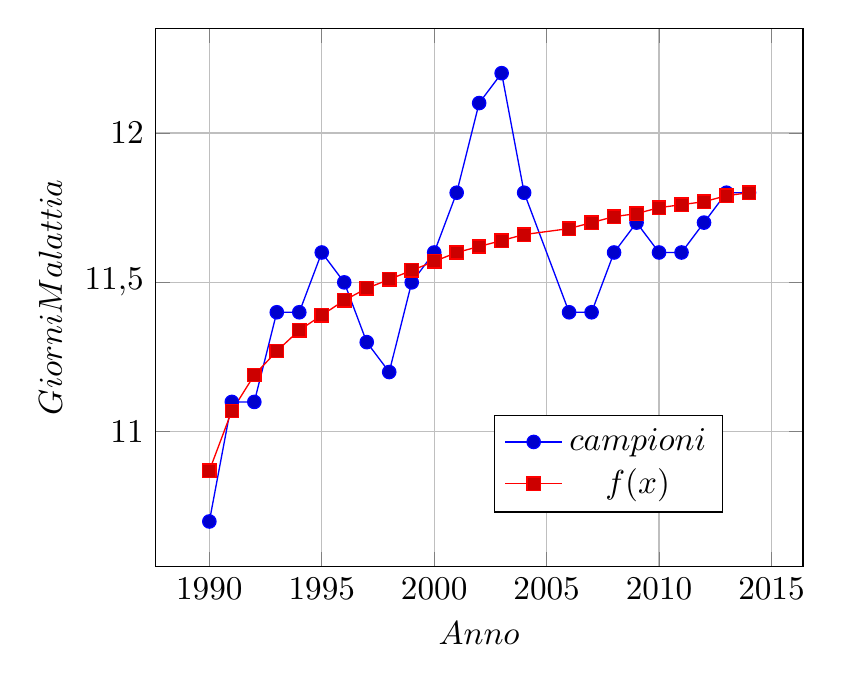
\begin{tikzpicture}[scale=1.2]
 \pgfkeys {
			/pgf/number format/.cd,
			set decimal separator={,{\!}},
			set thousands separator={}}
	\begin{axis}[ xlabel=$Anno$, ylabel=$Giorni Malattia$, grid=major, legend style={anchor=south, at={(0.7,0.1)}} ]
		
		\addplot coordinates{( 1990, 10.7) 
							  ( 1991, 11.1)
							  ( 1992, 11.1)
							  ( 1993, 11.4)
							  ( 1994, 11.4)
							  ( 1995, 11.6)
							  ( 1996, 11.5) 
							  ( 1997, 11.3)
							  ( 1998, 11.2)
							  ( 1999, 11.5)
							  ( 2000, 11.6)
							  ( 2001, 11.8)
							  ( 2002, 12.1)
							  ( 2003, 12.2)
							  ( 2004, 11.8)
							  ( 2006, 11.4)
							  ( 2007, 11.4)
							  ( 2008, 11.6)
							  ( 2009, 11.7)
							  ( 2010, 11.6)
							  ( 2011, 11.6)
							  ( 2012, 11.7)							  
							  ( 2013, 11.8)
							  ( 2014, 11.8)
							  };
							  
		\addplot coordinates{( 1990, 10.87) 
							  ( 1991, 11.07)
							  ( 1992, 11.19)
							  ( 1993, 11.27)
							  ( 1994, 11.34)
							  ( 1995, 11.39)
							  ( 1996, 11.44) 
							  ( 1997, 11.48)
							  ( 1998, 11.51)
							  ( 1999, 11.54)
							  ( 2000, 11.57)
							  ( 2001, 11.60)
							  ( 2002, 11.62)
							  ( 2003, 11.64)
							  ( 2004, 11.66)
							  ( 2006, 11.68)
							  ( 2007, 11.70)
							  ( 2008, 11.72)
							  ( 2009, 11.73)
							  ( 2010, 11.75)
							  ( 2011, 11.76)
							  ( 2012, 11.77)		
							  ( 2013, 11.79)
							  ( 2014, 11.80)
							  };
				\legend{$campioni$,$f(x)$}
	\end{axis}
\end{tikzpicture}

Quindi, si osserva che la nostra stima per l'anno 2016 di nostro interesse, il numero di giorni di malattia per singolo dipendente si assesta intorno ai:
 	
 \[		x = 26 \] 
 
( perche' il 2016 rappresenterebbe il 26 e-simo  valore nel nostro intervallo di campioni )
 \[		f(26) = 11,82 ( consideriamo 12 )	\]
 
consideriamo le seguenti ipotesi per ogni singolo centralinista: 
\begin{savenotes}
\begin{table}[htb]
\centering
 \caption{Assunzioni iniziali in un singolo mese}
 \begin{tabular}{p{7cm}D{,}{,}{5.2}}
 \toprule
 	& \multicolumn{1}{c}{\textbf{Quantita'}} \\
 \midrule 	
	\makebox[7cm][r]{Giorni lavorativi} & 18,50\\
	\makebox[7cm][r]{Giorni assenza} & 12,00\\	
 	\makebox[7cm][r]{Probabilita' di stipulare un contratto (\%)\footnote{dati istat}} & 15,60\\
 \bottomrule
 \end{tabular} 
\end{table}
\end{savenotes}
%
%	Numero chiamate centralinisti
%
\begin{savenotes}
\begin{table}[htb]
\centering
 \caption{Numero contratti centralinisti}
 \begin{tabular}{p{7cm}D{,}{,}{5.2}D{,}{,}{5.2}}
 \toprule
 	& \multicolumn{1}{c}{\textbf{Singolo Centralinisti}} & \multicolumn{1}{c}{\textbf{30 Centralinisti}} \\
 \midrule 		
	\makebox[7cm][r]{Numero chiamate giornaliere} & 94,00 & 2820\\
 	\makebox[7cm][r]{Numero chiamate mensili} & 1739,00\footnote{(94,00*18,50)} & 52170\\
 	\makebox[7cm][r]{Contratti stipulati mensilmente} & 271,29 & 8138,52\\ 	
 	\makebox[7cm][r]{Chiamate mensili in caso di assenza per 12 giorni} & 611,00\footnote{(94,00*(18,50-12,00))} & 18330\\
 	\makebox[7cm][r]{Contratti stipulati in caso di assenza per 12 giorni} & 95,32\footnote{(611*0,156)} & 2859,48\\ 	
 \bottomrule
 \end{tabular} 
\end{table}
\end{savenotes}

 
\begin{savenotes}
\begin{table}[htb]
\centering
 \caption{Variazione Fatturato}
 \begin{tabular}{p{8cm}D{,}{,}{5.2}D{,}{,}{5.2}}
 \toprule
 	& \multicolumn{1}{c}{\textbf{VAN PAREGGIO}} & \multicolumn{1}{c}{\textbf{VAN CASO REALE}} \\
 \midrule
 	\makebox[8cm][r]{Probabilita' di successo di un contratto (\%)} & 11,54 & 15,00\\
 \midrule
	\makebox[8cm][r]{Numero contratti stipulati (1 mese)} & 8138,52 & 8138,52\\
	\makebox[8cm][r]{Numero contratti stipulati (30 malati in 1 mese)} & 2859,48 & 2859,48\\
 \midrule	
	\makebox[8cm][r]{Numero contratti successo (1 mese)} & 939,50 & 1220,78\\
	\makebox[8cm][r]{Numero contratti successo (30 malati in 1 mese)} & 329,98 & 428,92\\
 \midrule	
	\makebox[8cm][r]{Fatturato Lordo (\euro) (1 mese)} & 75160,00 & 97662,40\\
	\makebox[8cm][r]{Fatturato Lordo (\euro) (30 malati in 1 mese)} & 26398,72 & 34313,76\\	
 \midrule	
	\makebox[8cm][r]{Fatturato Netto (\euro) (1 mese)} & 65314,04 & 84917,46\\
	\makebox[8cm][r]{Fatturato Netto (\euro) (30 malati in 1 mese)} & 22953,69 & 29835,81\\	
 \bottomrule
 \end{tabular} 
\end{table}\
\end{savenotes}